\chapter{Validation Methodology and Correctness}
\label{ch:validation}

A renderer that introduces a new sampling scheme (\Cref{ch:architecture}) has to be shown
correct before its speed means anything. The
sort-free analog-decomposition sampler is only useful if it produces the \emph{same} images a correct
volumetric path tracer would. The production optimisations of \Cref{ch:optimization} are only
admissible if they do not perturb that result. This chapter establishes that correctness. It first
explains \emph{how} the renderer is validated. No closed-form solution gives the correct image for these
scenes, so validation is \emph{differential}: two independent renderers are configured
identically and compared (\Cref{sec:reference-problem}). It then covers the statistics needed to compare two
stochastic renderers fairly (\Cref{sec:compare-correctly}). Next, it validates the renderer
on a sequence of increasingly
complex scenes, from a single Gaussian with a closed-form answer up to the full cloud, in absorption
(\Cref{sec:absorption-ladder}) and then in scattering (\Cref{sec:scattering-ladder}). It validates each
rendering feature against the reference (\Cref{sec:feature-validation}) and closes on the combined
showcase (\Cref{sec:money-shot}). Throughout, the scattering comparisons and the furnace
invariant (the albedo-one energy-conservation test of \Cref{sec:scattering-ladder}) serve as the
empirical \emph{unbiasedness evidence} for the analog-decomposition sampler. A
biased free-flight rule would shift the converged scattering result away from the energy-conserving
furnace value and from the independently-correct Mitsuba-analog reference (the reference run in its
unbiased analog mode, \Cref{sec:reference-problem}).

\section{Experimental setup}
\label{sec:setup}

All results in this thesis were measured on a single workstation, an NVIDIA GeForce RTX~3090 (Ampere,
compute capability~8.6, \SI{24}{\giga\byte}), with one explicitly-scoped exception noted below. The
renderer is built on CUDA and OptiX~9 in its release configuration (\texttt{-O3},
\texttt{-{}-use\_fast\_math}). The Mitsuba~3 reference runs on the same GPU through its CUDA backend, so
cross-renderer comparisons are on identical hardware. For the record: the validation host runs
CUDA~12.6 (NVIDIA driver 580.95 at the time of writing). The reference as shipped runs on the
Mitsuba build it was released against (Mitsuba~3.6.4), and the corrected-reference arms
(comparison configurations; conventions below) of
\Cref{sec:results-firefly} run on stock Mitsuba~3.8.0 with Dr.Jit~1.3.1. The lone exception is the Shader Execution
Reordering probe of \Cref{sec:ser}, which requires Ada-generation hardware and was therefore run on a
rented NVIDIA GeForce RTX~4090 (Ada, compute capability~8.9; CUDA~13.2, driver~595.58). Those figures are
marked throughout as a cross-architecture probe and feed into no 3090 result. Unless noted
otherwise, every timing figure is taken at a single fixed commanded operating point, to avoid
clock-throttling artefacts (\Cref{sec:compare-correctly}): \SI{350}{\watt} power
cap, SM (streaming multiprocessor, the GPU's compute core) clock pinned at
\SI{1800}{\mega\hertz}.\footnote{Under load the card sustains
\SIrange{1545}{1600}{\mega\hertz}; the pin caps the boost clock rather than preventing thermal pull-down.} The
equal-quality metric,
being a ratio, is robust to the operating point regardless. Every timing A/B additionally
\emph{interleaves} its two arms within each seed block (arm~A, arm~B, arm~A, \ldots) rather than running
one arm fully and then the other. Any residual clock or thermal drift thus affects both arms equally
and cancels in the comparison.

\paragraph{Measurement conventions.} The following conventions are used by every experiment in this
thesis; each experiment's setup refers back to them rather than re-deriving them.
\begin{itemize}
  \item \textbf{Seeds and budgets.} An \emph{arm} (one side of a comparison: a renderer--estimator
  configuration) written ``$n\times s$\,spp'' is the average of $n$ independent renders at $s$ samples per pixel (spp; effective budget
$n\cdot s$). Absorption
  renders in this renderer are \emph{deterministic}---the escape transmittance is analytic
  (\Cref{sec:analytic-od})---so they carry no seed variance and a single render suffices. Scattering
  renders are Monte Carlo, and every statistical statement about them uses multiple seeds.
  \item \textbf{Noise constant $k$.} The per-pixel variance of luminance across seed renders,
  multiplied by the spp. The multiplication removes the budget: an average of $s$ samples has
  variance proportional to $1/s$, so $k$ is the per-sample variance of the estimator itself. For
  an unbiased estimator it is constant in spp: it characterises the estimator, not the number of
  samples taken.
  Per-pixel variance also depends on the \emph{reconstruction filter}. This is the standard
  weighting that turns a pixel's samples into its final value; it is not a post-process and
  not a denoiser. Mitsuba's default filter (a Gaussian) spreads each sample over
neighbouring pixels;
  this renderer's box filter does not. A wider filter lowers per-pixel variance, so comparing
  $k$ across different filters would be meaningless. Every cross-renderer comparison in this
  thesis therefore uses the identical box filter on both arms. A firefly-robust variant, \emph{clip-99.9}, is used alongside it (fireflies: rare,
extremely bright outlier samples that dominate raw variance): the arm's seed stack is
clamped at its own \num{99.9}th-percentile luminance before $k$ is computed---a companion
number that fireflies cannot dominate. Where the raw and clipped values disagree substantially, both are reported.
  \item \textbf{Equal-quality speedup.} The fair speed question is: how much sooner does one
  renderer reach a chosen noise level? Noise per sample is $k$; time per sample is $t$.
  Reaching a target variance $v$ needs $k/v$ samples, which costs $t \cdot k/v$ seconds.
  The equal-quality speedup of renderer $B$ over renderer $A$ is therefore
  $(k_A t_A)/(k_B t_B)$. This is the only cross-renderer efficiency metric used in this
  thesis.
  \item \textbf{Confidence intervals.} Intervals on seed-derived ratios are \emph{bootstrap}
  intervals: the seeds are resampled with replacement many times, the statistic is recomputed
  each time, and the interval spans the middle \num{95}\,\% of the results.
  \item \textbf{Timing protocol.} Locked clocks (\SI{350}{\watt} power limit, SM clock pinned); one
  warm-up render absorbs just-in-time (JIT) kernel compilation; then five steady-state repeats, reported as the
  median with the spread stated. Wall-clock time is the primary measure because it applies
  identically to both renderers and is what a user experiences. As a cross-check, Dr.Jit's
  \emph{kernel history}---the reference's own benchmarking method---agrees with it to
  \num{0.15}\,\%: kernel-only \num{416.6} versus
  wall-clock \num{417.2}\,ms per sample.\footnote{Measured on the reference's \num{256}-spp
  showcase timing renders; the kernel history sums the GPU execution time of every launched
  kernel.} No compilation or host-side
  cost therefore hides in any reported time. Timed arms are interleaved.
  \item \textbf{Difference maps.} Signed relative difference panels share one convention:
  red where this renderer is brighter than the reference, blue where darker, white at
  agreement; each caption states its full scale.
  \item \textbf{Metrics on raw radiance.} Every root-mean-square error (RMSE), mean ratio,
and signed difference in this thesis is computed on the raw high-dynamic-range (HDR)
radiance values, \emph{before} any tonemapping or gamma (the nonlinear compressions that
map HDR radiance into displayable pixel values). Saturated
  display regions (a white background, a black interior) thus cannot conceal a discrepancy from the
  metrics, even where they conceal it from the eye. Mean ratios are this renderer over the
reference unless stated otherwise.
  \item \textbf{Budget policy.} For all rendered-artifact comparisons, the scene is matched exactly
  and each arm receives whatever sample budget pushes its own noise below the systematics being
  resolved. The arms' budgets therefore differ. Per-sample efficiency is compared only in the
  dedicated equal-quality figures (\Cref{sec:results-perf}).
\end{itemize}

\section{Differential validation}
\label{sec:reference-problem}

Multiple scattering in an arbitrary Gaussian mixture has no closed-form solution. There is
therefore no exact image to compare against for these assets. Correctness is instead
established \emph{differentially}: a second, independent renderer is configured identically,
and the two outputs are compared quantitatively.

The reference is Mitsuba~3~\cite{Mitsuba3}, configured identically, primitive for primitive,
from the same Gaussian data. Mitsuba is mature and widely trusted, and it solves the same
volumetric light-transport integral. A small difference that shrinks with sample count is
therefore strong evidence of correctness. A structured difference localises a bug. This turns
an unfalsifiable ``does it look right?'' into a measurable gap, and it is the backbone of
every result below. Two configurations are the exceptions; they have exact answers. A single Gaussian in
absorption has a closed-form transmittance (\Cref{sec:absorption-ladder}). In the furnace
configuration---an albedo-one medium inside a unit-radiance environment---every pixel must
equal exactly one (\Cref{sec:scattering-ladder}). In these two cases the renderer is checked
against the exact value; Mitsuba is not involved.

\paragraph{A reference is only as good as its configuration.} A reference image is a valid
target only if we know exactly how it was produced. The integrator used matters most.

Each asset ships with pre-rendered images (\texttt{reference\_pyrN},
\texttt{optimized\_pyrN}), provided by the reference's authors. These images come from the
\emph{fitting} pipeline: the optimisation that fit the Gaussians to the source volume, not a
path tracer. The \texttt{optimized} images render the
fitted Gaussians with the fit's own forward model, a \emph{tomographic} integrator
(\texttt{volprim\_tomography}).\footnote{Established from the release itself: its
asset-generation scripts invoke \texttt{volprim\_tomography}, and re-rendering the fitted
Gaussians with that integrator reproduces the bundled images (recorded in the repository's
development log).}
Tomography integrates density along straight camera rays and shows the background
attenuated by it; there is no scattering, and light never changes direction. Absorption rendering shares that no-scattering form, but the two integrate different
media. Absorption uses the radiometric convention: normalised, support-truncated kernels
at the calibrated scale. Tomography uses the fit's raw convention: each Gaussian's stored
weight is its peak density, integrated over the full line. The normalisation depends
on each Gaussian's size, so no single density multiplier converts one convention into the
other. The \texttt{reference} images do not show the
fitted Gaussians at all; they show the fit's target, the source volume, and the radiometric
gap is large. The bundled images average \num{0.55} over their \num{36} views (range
\numrange{0.40}{0.77}), re-measurable directly from the shipped file
(\texttt{optimized\_pyr0.exr}). Path-traced renders of the same
primitives converge near \num{0.32} (\Cref{sec:scattering-ladder}). The two
conventions---tomographic projection and path-traced light transport---differ by roughly
$1.7\times$ before either renderer is even in question.

Those images are the obvious first calibration target, and matching them by tuning the
density scale would be a mistake for two reasons: it would use a density change to
compensate for an integrator difference, and it would fold the fit's own approximation
error into the renderer's calibration.
Every comparison in this chapter instead uses references regenerated under the renderer's own
configuration: the same integrator, the same $\sigma$ scale, the same camera and
lighting,\footnote{The \emph{density scale}---written ``$\sigma$ scale'' or ``$\sigma_t$
scale'' and set by \texttt{-{}-sigma-multiplier}---is a single global multiplier on every
primitive's extinction. It is unrelated to the standard deviation $\sigma$ of the
$3\sigma$ support (\Cref{sec:kernel-mixture}).}
matched primitive for primitive. Geometry is exact on both sides: every banked reference
arm---the cloud scene package, the asset harness, and the furnace probes---runs Mitsuba's
analytic \texttt{ellipsoids} shape, the counterpart of this renderer's analytic sphere.

One level deeper, the implementation \emph{revision} matters as much as the
configuration. As \Cref{sec:results-firefly} documents, even the configuration-matched reference
required diagnosis and correction~\cite{KramarzVolprimFixes2026} before its fast estimator could serve
as a target. Every comparison in this thesis therefore states which reference revision it was made
against and, where applicable, which correction set. One naming convention is used throughout.
\emph{The reference as shipped} is the \texttt{volumetric\_primitives} revision released with
DSYG~\cite{DSYG}: the code as its users obtain it, and the revision the benchmarked comparisons of
\Cref{ch:results} were made against. (\texttt{volprim}, as its integrators are named, abbreviates
\texttt{volumetric\_primitives}.) \emph{The current upstream revision} is the newer
\texttt{GaborVolumes} codebase. \emph{Corrected} marks a revision with the correction set of
\Cref{sec:results-firefly} applied. (\Cref{tab:revision-timeline} places the three revisions on a
timeline.) Separately, a ``shipped \emph{configuration}'' refers to a
code's default runtime settings. For the reference that notably includes its shadow-march
early-out, enabled by default: its shadow rays stop marching past a fixed optical depth
(\Cref{sec:results-firefly}). Two further conventions are used from here on. The binding
\emph{analog} names the
configuration that gathers direct light only when a path escapes to the environment, with no
next-event estimation. This is the reference's unbiased mode (\Cref{sec:nee-mis}). Comparison arms
are labelled \emph{this renderer (MIS)}, \emph{reference (analog)}, and \emph{reference (corrected
NEE)}.

\subsection{An independent integrator: a voxel-grid cross-check}
\label{sec:voxel-gt}

The Mitsuba comparison shares one assumption with this renderer: both treat the medium as a
sum of analytic Gaussians. An error in that shared closed form could, in principle, survive
in both renderers at once. A stronger check removes the assumption: the same medium is
rendered by a route that never touches the Gaussian closed form, and the two results are
compared. The Gaussian field is baked into a dense voxel grid in the renderer's own,
mass-conserving density convention,
\[
  \sigma_t(\mathbf{x})=\sum_i M_i\,(2\pi)^{-3/2}\!\prod_j s_{ij}^{-1}\;
  \exp\!\big(-\tfrac12\lVert S_i^{-1}R_i^{\!\top}(\mathbf{x}-\boldsymbol\mu_i)\rVert^2\big),
\]
and that grid is rendered by Mitsuba's \texttt{heterogeneous}/\texttt{gridvolume} path tracer
via delta tracking. That code path shares no code and no Gaussian mathematics with either
analytic renderer.

In absorption the cross-check succeeds (\Cref{fig:voxel-gt}). Absorption is the right regime
for it: the image depends only on transmittance, so no scattering variance enters. At
production density, through the opaque interior and the empty
background, the grid render matches the analytic render to a median pixel difference of
${\sim}2\times10^{-5}$. Deep in the core that agreement is easy, since both arms are
near-black there; the bottom row of \Cref{fig:voxel-gt} therefore repeats the cross-check at
\num{4}\,\% density (the reduced-density protocol of \Cref{sec:absorption-ladder}), where
nothing saturates. At production density one residual is visible: a thin band at the silhouette.

The band is the grid's own discretisation error. A grid stores one density value per voxel,
so it blurs the Gaussians' edge falloff, and rays that graze the silhouette accumulate
slightly different optical depth than against the exact form. Two observations attribute the
band to the grid: refining the grid shrinks it and moves the grid's image mean toward the
analytic one,\footnote{From $128^3$ to $600^3$:
band RMSE $0.072\!\to\!0.057$; image means $0.394\!\to\!0.401$, analytic \num{0.416}.}
while adding samples barely moves it.\footnote{Quadrupling \num{32}\,spp to \num{128}\,spp
changes an intermediate $200^3$ grid's band RMSE from \num{0.0627} to \num{0.0613}.}
As the voxels shrink, the grid render converges to the analytic one; the cross-check thus
supports the renderer's correctness, and it also quantifies the
edge fidelity gained by the analytic primitive over a voxelised proxy. At \num{4}\,\%
density the same error is visible in full rather than only at the edge: the signed
difference in the bottom row of \Cref{fig:voxel-gt} is the high-pass residual of the grid's
smoothing---the analytic render is darker in the fine wisps the grid blurs away, brighter in
the gaps between them---with mean ratio \num{1.0079} and RMSE \num{0.017}, more than five
times the grid arm's measured noise floor of \num{0.003} (two seeds at \num{4096}\,spp).

Scattering is deliberately not cross-checked this way. Delta tracking needs a
\emph{majorant}: a known upper bound on the density inside a region. This medium's density
spans orders of magnitude, which makes any majorant a bad one. A single global bound rejects
almost every tentative collision, and the images drown in fireflies. A coarse per-block bound
risks undershooting a peak, which biases the result. Either failure would swamp the
comparison. Scattering correctness therefore rests on the furnace invariant
(\Cref{sec:scattering-ladder}) and the Mitsuba-analog comparison.

\begin{figure}[htp]
  \centering
  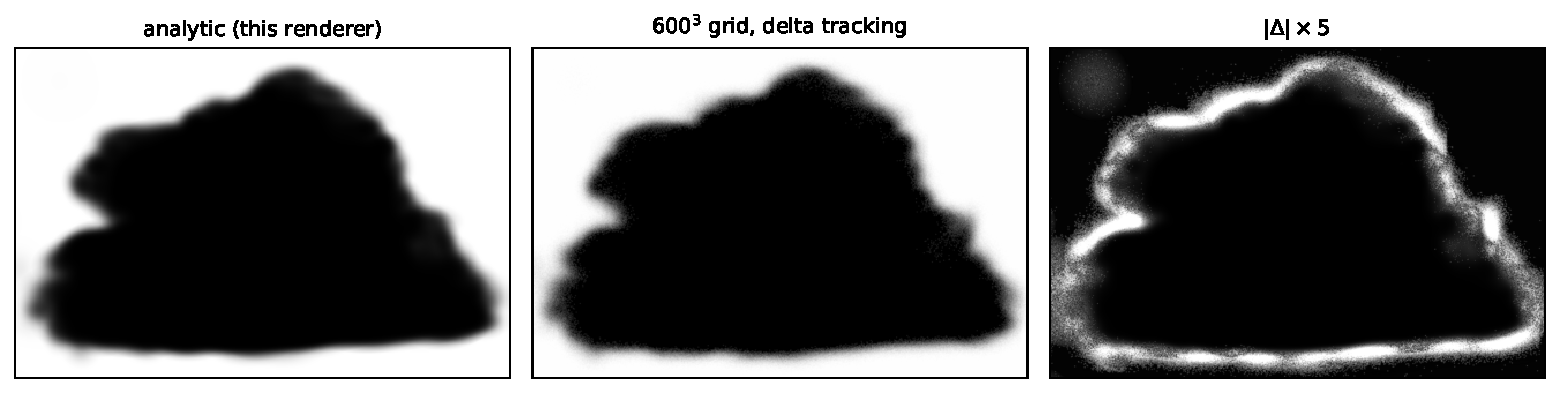
\includegraphics[width=\linewidth]{figures/voxel_gt.pdf}
  \caption{Independent voxel-grid cross-check (cloud, absorption, same camera).
\emph{Top row, production density}: the analytic Gaussian renderer; the same density field
baked to a $600^3$ grid and rendered by Mitsuba's dense-grid delta-tracking path tracer
(\num{32}\,spp); absolute difference at $5\times$ gain, gamma-mapped (white ${=}$
$|\Delta|\ge0.2$). Interior and background match to a median pixel difference of
${\sim}2\times10^{-5}$; the only visible residual is the silhouette band where the grid
blurs the sharp Gaussian boundary. \emph{Bottom row, \num{4}\,\% density} (the
reduced-density protocol of \Cref{sec:absorption-ladder}; grid arm unclamped,
\num{4096}\,spp): with the whole interior visible, the same blur appears everywhere as the
structure of the signed difference ($\pm\num{5}\,\%$ full scale; conventions,
\Cref{sec:setup}). The analytic arms agree at the noise level under this protocol
(\Cref{fig:reduced-density}), so this structure is the grid's discretisation, not
renderer disagreement (mean ratio \num{1.0079}; discussion in the text).}
  \label{fig:voxel-gt}
\end{figure}

\section{How to compare correctly}
\label{sec:compare-correctly}

Comparing two Monte~Carlo renderers is itself error-prone, and several pitfalls had to be controlled.
\emph{Bias and variance must be separated.} A single per-pixel RMSE between two noisy renders conflates
estimator \emph{bias} (a systematic difference that survives convergence) with \emph{variance} (noise
that vanishes as samples grow). Concretely, for two independent renders $A$ and $B$ of the same scene,
the expected per-pixel squared difference splits cleanly into the two,
\[
  \mathbb{E}\big[(A-B)^2\big]
  = \underbrace{\big(\mathbb{E}[A]-\mathbb{E}[B]\big)^2}_{\text{bias}^2}
  + \underbrace{\operatorname{Var}[A]+\operatorname{Var}[B]}_{\text{noise}}.
\]
A single raw difference therefore cannot, on its own, tell a genuine discrepancy from sampling noise.
Re-rendering each image under several independent seeds estimates the noise term directly (as the
inter-seed variance). When the measured difference is statistically consistent with that noise floor,
the bias term is zero to within the noise. This is the sense in which two renders are said
here to
``match to within Monte~Carlo noise.'' The renderer is therefore checked for bias by comparing \emph{converged} means. Each arm is
averaged over enough seeds and samples that its own residual noise sits far below the
difference under test. Where an analytic value exists, the mean is compared to it directly.
Efficiency is a separate question, and it is compared only at \emph{equal quality}: one
renderer is faster than another only if it reaches the same noise constant $k$ in less time,
under the conventions of \Cref{sec:setup} (the definition of $k$, the firefly-robust
statistics, and the fixed GPU operating point). Raw frame times at a fixed sample count are
reported only alongside this equal-quality figure (\Cref{ch:results}).

\section{Absorption: from a single Gaussian to the full cloud}
\label{sec:absorption-ladder}

With scattering disabled (albedo $0$), the image depends only on transmittance, which for a Gaussian
mixture is the closed-form optical depth of \Cref{sec:analytic-od}---so the ground truth is
\emph{analytic}, independent of any reference renderer. This isolates the geometry and the optical-depth
integration from the stochastic scattering logic.

\paragraph{Single Gaussian.} \textbf{Goal:} verify the ray--primitive transform, the erf-based
optical depth, and the camera model against an exact answer.

\textbf{Setup:} one unit Gaussian,
absorption only; the expected transmittance at every pixel is evaluated from the closed form of
\Cref{sec:analytic-od}---no reference renderer is involved, and the render is deterministic
(\Cref{sec:setup}).

\textbf{Result:} converged per-pixel RMSE of $\sim\!2\times10^{-5}$ against the
closed form (\Cref{fig:absorption-ladder}; mean ratio $1.0000$, i.e.\ no systematic offset).

\paragraph{Overlapping primitives.} \textbf{Goal:} verify two things the single-Gaussian stage
cannot. First, the optical depths of overlapping primitives must \emph{add} correctly along a ray.
Second, the hit collection must track simultaneously-overlapping primitives without losing
any (the same active set the scattering sampler of \Cref{sec:adt} later draws from).

\textbf{Setup:} two overlapping Gaussians compared against Mitsuba under the matched
configuration; plus a deliberately degenerate \emph{collinear} stress test---$m$ identical Gaussians
stacked in place.

\textbf{Result:} the plotted pair is compared against Mitsuba: up to the active-set
capacity, the renderer matches the reference for the combined medium to $\sim\!10^{-4}$ in
the mean. Additivity itself is checked analytically, by the collinear test: $m$ identical
Gaussians stacked in place are exactly one $m$-fold-denser Gaussian, so the ground truth is
the closed form. That test goes unplotted because its correct image is indistinguishable
from the single-Gaussian stage's.

Pushed past capacity, the collinear test exposed a silent failure. The active set has a fixed
capacity; past it, old revisions dropped primitives without any warning, and the image stayed
plausible. The mechanism was still identifiable from the image alone. With $m$ stacked Gaussians sharing
a total optical depth $\tau_0$, keeping only $\text{cap}$ of them integrates the fraction
$\min(\text{cap},m)/m$ of that depth. The measured transmittance matched
$\exp(-\min(\text{cap},m)/m\cdot\tau_0)$ to $10^{-4}$: the image alone revealed that
primitives were being dropped, and how many. After the capacity fix, all $m$ match the analytic answer to
$2.3\times10^{-4}$ (\Cref{sec:gpu-impl}).

The same stress test surfaced a \emph{reference} limitation. Mitsuba's volumetric-primitive
integrator under-absorbs when identical primitives are stacked. At fixed total mass, its
centre transmittance reads $0.278$ at $m{=}40$ and $0.447$ at $m{=}64$; the exact value is
$0.205$, which this renderer matches to $2.3\times10^{-4}$. The deviation grows monotonically
as the same mass fragments across more primitives. The reading is statistically solid: it
is taken at the image centre, through the stack's deepest line of sight, and the deviation
there is two orders of magnitude above the Mitsuba arm's residual noise (this renderer's
values are deterministic). It is also practically narrow: perfectly collinear stacking is a
degenerate configuration that real assets never reach, so it does not affect the
scene-level comparisons. It does show that a differential comparison can inherit the
reference's own errors, which is why the analytic check is the arbiter for this stage.

\paragraph{The cloud.} \textbf{Goal:} absorption correctness at scene scale. Scattering stays
disabled, so this stage still has an exact transmittance check.

\textbf{Setup:} the full \num{652}-primitive Disney cloud, the headline asset throughout
this thesis (Gaussians fit to the Disney/WDAS cloud volume~\cite{WDASCloud2017}). It is rendered from all
\num{24} camera views against Mitsuba (the reference arm at \num{1024}\,spp per view; this
renderer's absorption arm is deterministic). On one representative view, the exact transmittance is additionally computed by brute
force: every pixel's closed-form optical depth is summed over all \num{652} primitives in
float64. This third, independent computation settles whether the edge band belongs to this renderer or to the reference's noise.

\textbf{Result:} across all \num{24} views
the aggregate mean transmittance difference is $+1.6\times10^{-5}$ (worst view
$7.8\times10^{-5}$), with a per-pixel RMSE of \num{0.0094} dominated by the reference arm's
residual Monte-Carlo noise. On that view, \num{93}\,\% of the visible silhouette band is the
reference arm's Monte-Carlo noise; the remainder is zero-mean at the ${\sim}2\times10^{-3}$
level. The same brute-force arm also confirms agreement in the \emph{optical-depth} domain,
where deep-$\tau$ errors would be magnified rather than compressed: on the represented view,
this renderer matches the float64 computation to a transmittance RMSE of $9.5\times10^{-5}$
and a mean optical-depth ratio of \num{0.9999}, with a median per-pixel relative
optical-depth error of \num{0.05}\,\% (pixels with $T$ between $10^{-3}$ and \num{0.999};
both arms deterministic, so the comparison carries no Monte-Carlo noise at all).
\Cref{fig:absorption-ladder} collects the three stages.

\begin{figure}[htp]
  \centering
  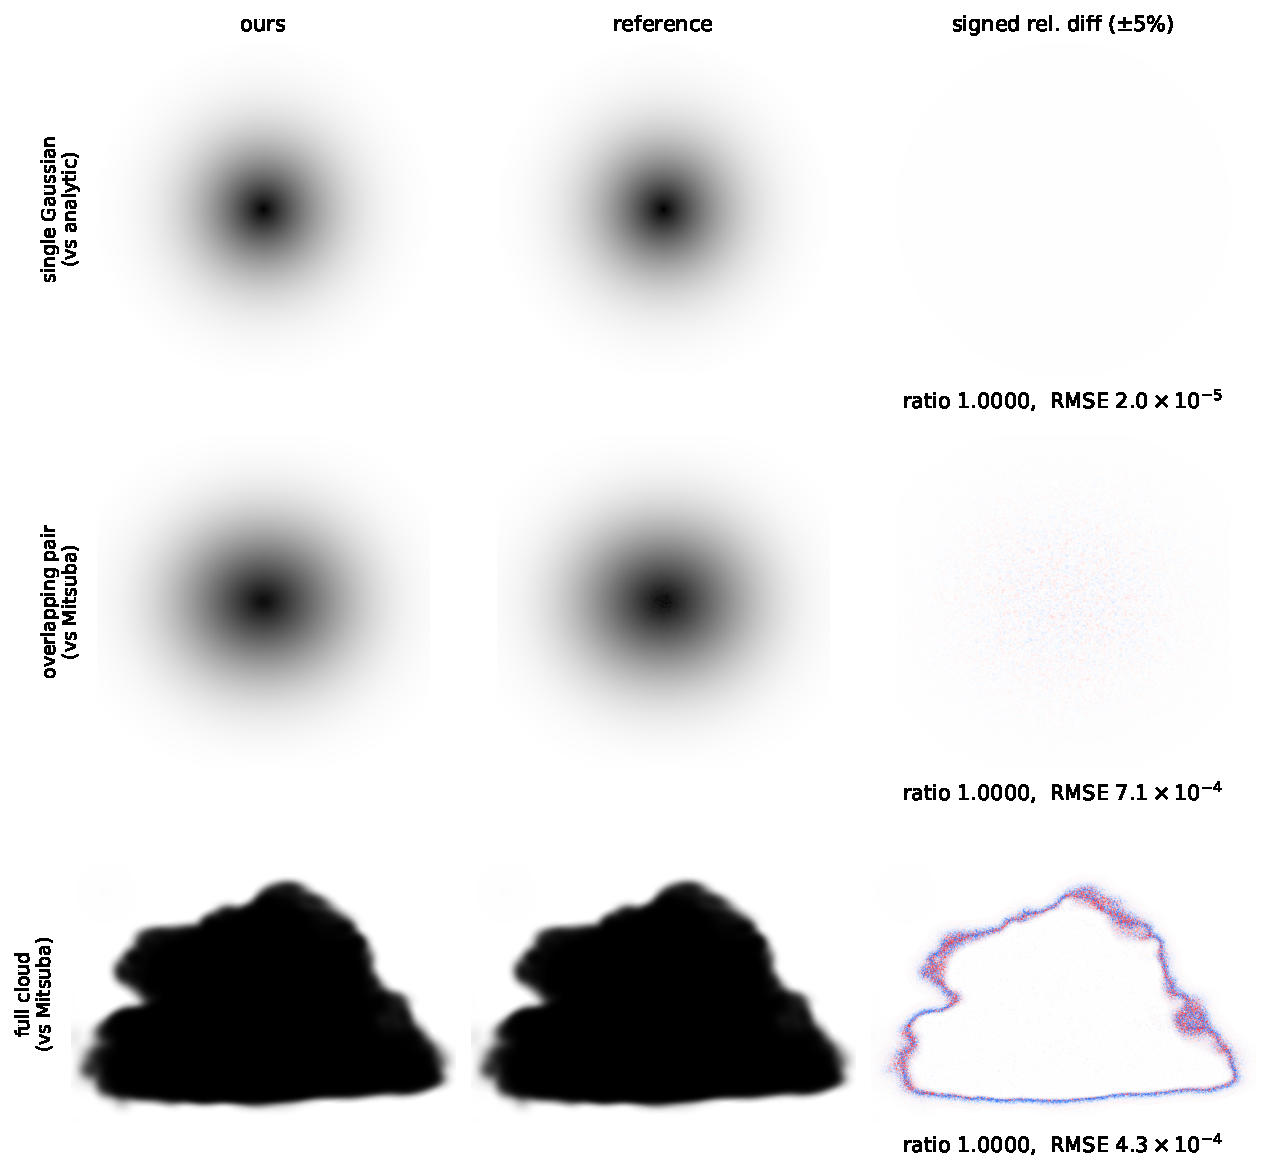
\includegraphics[width=\linewidth]{figures/absorption_ladder.pdf}
  \caption{Absorption-only validation in three stages: a single Gaussian, an overlapping
pair, and the full \num{652}-primitive cloud, each annotated with its converged-mean ratio (this
renderer over the stage's ground-truth arm) and per-pixel RMSE. The single Gaussian is held to its closed-form transmittance (agreement
$\sim\!2\times10^{-5}$; the closed form integrates the same $3\sigma$ support, isolating
numerical agreement from truncation). The pair and cloud are compared against Mitsuba, with
additivity checked analytically via the collinear test and the cloud's edge band resolved by
the float64 check of \Cref{sec:absorption-ladder}. Reference arms: \num{16384}\,spp
effective (pair) and \num{49152} (cloud), so the residual RMSE (\num{0.0007}, \num{0.0004})
is systematic rather than noise; this renderer's panels are noise-free (analytic
transmittance). Render panels are tonemapped for display only; every quoted number is
computed on raw radiance. At this density the cloud's core is opaque, so its panel is
black---\Cref{fig:reduced-density} repeats the comparison with the whole interior
visible. Difference panels: $\pm\num{5}\,\%$ full scale (conventions,
\Cref{sec:setup}).}
  \label{fig:absorption-ladder}
\end{figure}

\paragraph{The cloud at reduced density.} \textbf{Goal:} remove the display's blind spot. At
production density the cloud's core is optically deep, so the transmittance image is black
there---and a black pixel can hide any interior error, since below $T\approx10^{-3}$ even a
large relative error in optical depth no longer changes the pixel visibly. The float64
optical-depth check above addresses this in the metric domain; this stage addresses it in the
image itself, by repeating the comparison at a density where the whole interior is visible.

\textbf{Setup:} the same asset, camera, and arms as the cloud stage, with the density
multiplier reduced from the production \num{7.5} to \num{0.3} (\num{4}\,\% of production). The
deepest pixel then still transmits $T=\num{0.17}$, so every part of the volume stays in the
display's responsive range. The reference arm runs its analog estimator (unbiased in every
revision, \Cref{sec:results-firefly}), averaged over \num{12} seeds of \num{4096}\,spp---%
\num{49152} effective, the same budget as the cloud stage's reference arm; this renderer's
arm is deterministic.

\textbf{Result:} mean ratio \num{0.9999}; per-pixel RMSE \num{0.0010}, of which the reference
arm's own Monte-Carlo noise, measured across its seeds, accounts for \num{0.0009}; the mean
optical-depth ratio is \num{1.0003}. The difference panel of \Cref{fig:reduced-density} shows
no spatial structure: with nothing hidden by black, the interior agrees everywhere at the
noise level.

\begin{figure}[htp]
  \centering
  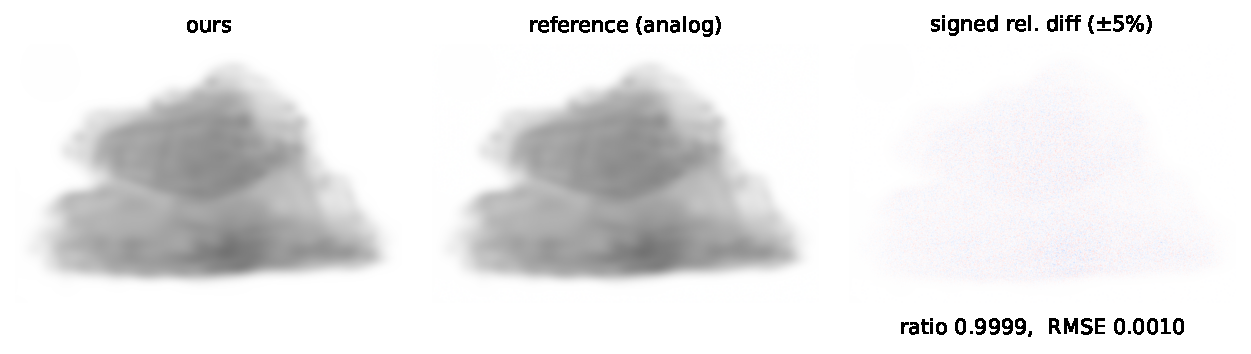
\includegraphics[width=\linewidth]{figures/reduced_density.pdf}
  \caption{The cloud at \num{4}\,\% of production density (multiplier \num{0.3} against the
production \num{7.5}): this renderer, the reference's analog arm (\num{12} seeds
$\times$ \num{4096}\,spp), and the signed relative difference. The darkest pixel transmits
$T=\num{0.17}$, so no interior error can hide in black; the render panels are a plain gamma
tonemap with no contrast stretch. Mean ratio \num{0.9999}, per-pixel RMSE \num{0.0010}
against a reference noise floor of \num{0.0009}. Difference panel: $\pm\num{5}\,\%$ full
scale (conventions, \Cref{sec:setup}).}
  \label{fig:reduced-density}
\end{figure}

\section{Scattering: from the furnace test to the full cloud}
\label{sec:scattering-ladder}

Enabling scattering (albedo $>0$) activates the full path tracer: the analog-decomposition sampler, the
phase function, and next-event estimation over many bounces. There is no closed-form image here, so two
checks are used: a reference-free energy invariant, and the differential comparison against Mitsuba.

\paragraph{Furnace test.}\label{par:furnace} \textbf{Goal:} a reference-free bias check. A medium
that absorbs nothing (albedo $1$), inside an environment radiating $1$ (uniform white) from every direction, can
only \emph{redirect} light. Redirecting light that is identical in all directions changes
nothing. The medium is therefore radiometrically invisible, and every pixel of a correct render must
equal
exactly $1$. In estimator terms, every path keeps its full energy at every interaction and
eventually escapes into the unit environment, returning exactly $1$. Any deviation of the mean from
$1$ is therefore estimator bias---no reference render, asset, or density scale enters.

\textbf{Setup:} \Cref{fig:furnace-four} runs this
invariant across the four estimator arms of this thesis' comparisons: this renderer with and
without its MIS direct lighting, and the reference's corrected next-event and analog modes. Each
arm runs over a
\num{64}-fold range of sample counts, two optical densities ($\sigma{=}6$, $\sigma{=}12$), and
\num{8} seeds per point.

\textbf{Result:} every arm holds the analytic value within its confidence
interval at every sample count. An unbiased estimator's mean equals the ground truth at any sample count; more samples
only shrink the scatter around it. The evidence is therefore the whole flat line rather than any
single point. The \emph{shipped} next-event estimator, by contrast, violated the invariant
by the same amount at every sample count: $+\num{9.7}\,\%$ centre over-count at
$\sigma{=}6$, $+\num{31}\,\%$ at $\sigma{=}12$.\footnote{Flat from \num{64} to \num{16384}\,spp at
$\sigma{=}6$ and to \num{4096}\,spp at $\sigma{=}12$ (the recorded sweep's ranges), and
depth-invariant---a bias, not undersampling.} That deviation triggered the diagnosis and
corrections
documented in \Cref{sec:results-firefly}. The bias was a property of that released implementation,
not of next-event estimation as a method; the corrected implementation passes the same invariant
(\Cref{fig:furnace-four}).

\begin{figure}[htp]
  \centering
  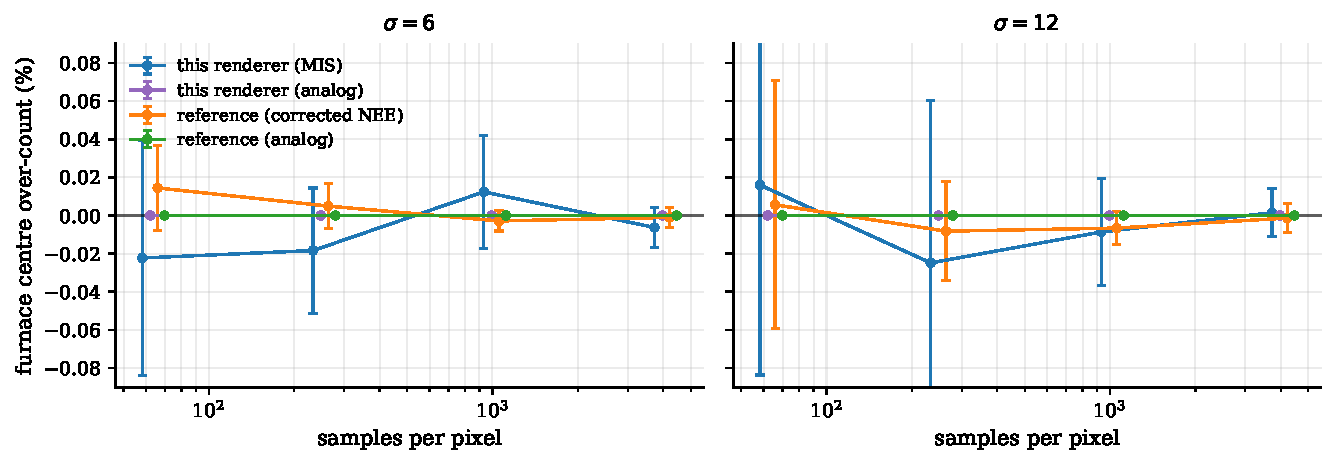
\includegraphics[width=\linewidth]{figures/furnace_four.pdf}
  \caption{Furnace test: centre over-count versus sample count for the four estimator arms, at density
scales $\sigma{=}6$ and $\sigma{=}12$ (single Gaussian, albedo $1$, uniform unit-radiance
environment; every pixel of a correct render equals exactly $1$, so the centre over-count is
the estimator bias; ``centre'' is the mean over the image's central quarter-box). All four
arms sit on $0$ at every sample count (error bars: \num{95}\,\% $t$-intervals over \num{8}
seeds; the widest low-sample intervals extend past the axis range). The two analog arms are \emph{exact} zeros with no spread: an analog furnace path
never changes weight, so every sample is exactly $1$. The reference's next-event arm passes because it carries the corrections of
\Cref{sec:results-firefly}; as shipped it does not pass this invariant (body text).}
  \label{fig:furnace-four}
\end{figure}

\paragraph{The scattering stages.} \textbf{Goal:} validate the full stochastic path tracer against
an independent implementation, through the same progression of scenes as absorption.

\textbf{Setup:} a single
scattering Gaussian, clusters, and the full cloud, each at albedo $0.9$, this renderer versus
Mitsuba-analog under the matched configuration; the compared quantities are converged means over
multiple seeds (\Cref{sec:setup}).

\textbf{Result:} the single-Gaussian stage
matches to within noise. The cluster and cloud stages match in the bulk but leave one small,
convergence-stable residual in the \emph{overlap} region. It is a $+2\times10^{-4}$ core difference on the
cluster, well outside that stage's recorded seed spread.\footnote{The early record preserved
the spread-based significance readout (${\sim}6$ standard errors) but not the seed count
behind it.} The same effect appears as ${+}1\times10^{-4}$ in the densest part of the cloud.
It is below $0.2\%$ of the peak and confined to vertices where many primitives overlap. It is \emph{not} a single-precision inversion artefact: replacing the float
$\operatorname{erf}^{-1}$ with a double-precision one moves the converged cluster mean by
${\sim}2\times10^{-8}$, four orders of magnitude below the residual. The two implementations therefore handle heavy overlap slightly differently from each other;
which one is wrong is unknown. Candidates on this side are the float-precision behaviour of the argmin rule when
many primitives overlap (near-coincident draws and entry points, \Cref{sec:adt}) and the
shadow-ray transmittance leaving a vertex \emph{inside} overlapping primitives. The
reference's side had overlap-regime issues of its own, later found and corrected
(\Cref{sec:results-firefly}); this record predates those fixes. The residual is therefore
carried unattributed: small, bounded, and stable under convergence. Everywhere else the
stages agree at the noise level.

Under the meadow illumination (``meadow'' throughout is the \texttt{meadow\_2} map;
\Cref{sec:money-shot} specifies it fully) the three arms' converged image means agree pairwise to within \num{1}\,\%.\footnote{This renderer: \num{0.3215} ($\pm\num{0.00001}$; the \num{18}-render
spp-weighted pool of \Cref{fig:g1-bias}, \num{40960}\,spp effective). Reference (analog):
\num{0.3201} ($\pm\num{0.004}$; \num{16}$\times$\num{64}\,spp, by far the noisiest arm).
Reference (corrected NEE): \num{0.3231} ($\pm\num{0.00003}$; \num{4}$\times$\num{2048}\,spp).
Each uncertainty is the standard error of the mean, estimated from that arm's own seed
spread.} This renderer's mean differs from the unbiased analog arm's by a third of that arm's
own statistical uncertainty ($0.35$ standard errors): as far as the analog arm can measure,
the two means are the same. This agreement of means is the unbiasedness evidence for the sampler. The two
tightly-converged arms resolve a genuine ${\sim}0.5\,\%$ offset against each other---the same
core-level systematic the pixel-level certification below localises and bounds. (Converged
means are estimator-independent, so this three-way comparison is an apples-to-apples check.)

The
${\sim}10^{-4}$ figure belongs to the \emph{localised} overlap residual above, not to the image
means. The reference arm in these comparisons is the analog mode, the shipped code's unbiased
configuration; the \emph{fast} (next-event) estimator is compared too, in its corrected
revision---immediately below at pixel level, and at equal quality in \Cref{sec:results-perf}
(\Cref{tab:likeforlike}).

\paragraph{Convergence to a common ground truth.} \textbf{Goal:} show that each renderer's RMSE against a converged render falls at the
Monte-Carlo rate, all the way to zero.

\textbf{Setup:} on the full showcase (\Cref{sec:money-shot}), each renderer is rendered at \num{16}--\num{4096}\,spp with
\num{4} independent seeds per budget. Its relative RMSE is measured against its own high-budget
ground truth, with seeds disjoint from every budget's, so no correlated noise enters. The ground truth's own residual noise, estimated from its seed spread, is subtracted, so the
error curves can fall to zero rather than floor at the ground truth's noise.

\textbf{Result:} \Cref{fig:nee-convergence}. Both estimators follow the exact Monte-Carlo
$-\tfrac12$ slope over \numrange{16}{4096}\,spp, with no error floor: the curves keep
falling rather than flattening at a residual level, which is what bias would
produce.\footnote{This renderer
$\num{106.6}\to\num{6.6}\,\%$; the reference $\num{92.8}\to\num{5.8}\,\%$. Every step ratio
matches the ideal $-\tfrac12$-slope prediction to within \num{1}\,\%.} At every budget, the
measured error equals the independent inter-seed noise estimate. Both observations are
consistent with an unbiased estimator; no unexplained residual remains. The reference arm
here is its \emph{corrected} next-event estimator; \Cref{sec:results-firefly} gives the
full account of the corrections.

\begin{figure}[htp]
  \centering
  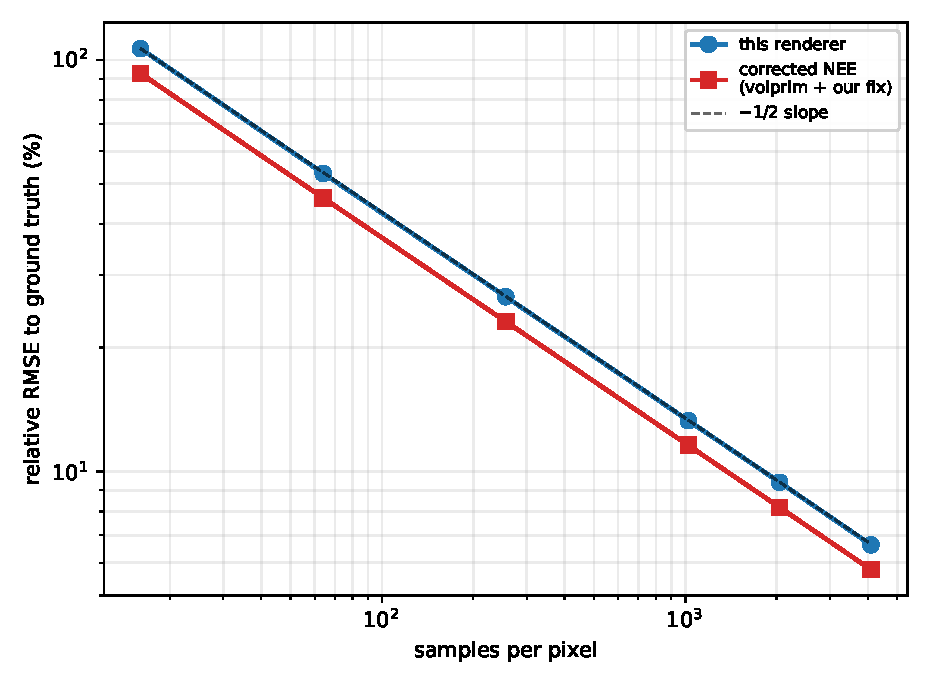
\includegraphics[width=\linewidth]{figures/nee_convergence.pdf}
  \caption{Error-to-ground-truth convergence on the cloud--meadow showcase: relative RMSE versus
  sample count (log--log) for this renderer's MIS estimator and the reference's corrected next-event
  estimator~\cite{KramarzVolprimFixes2026}, \num{4} independent seeds per point (ground truths:
  \num{12288}\,spp effective ours, \num{8192} reference, seeds disjoint from every budget;
  GT-noise-corrected). Both arms follow the exact $-\tfrac12$ Monte-Carlo slope with no error
  floor, and the measured error matches the inter-seed noise at every budget: both estimators are
  unbiased and converge to their common answer.}
  \label{fig:nee-convergence}
\end{figure}

\paragraph{Pixel-level cross-renderer agreement.} \textbf{Goal:} the stages above compare image
\emph{means}, and two images can share a mean yet disagree locally. This test therefore checks
the agreement pixel by pixel, everywhere in the frame.

\textbf{Setup:} converged averages on
the showcase under two lighting regimes. Under the peaky meadow, this renderer's
\num{8}$\times$\num{1024}-spp average is compared against the reference's \num{4}$\times$\num{2048}-spp corrected next-event
average: the same \num{8192}-spp effective budget on both sides, split into more, smaller
seeds on the cheaper arm (the noise prediction below needs several independent seeds). Under a uniform environment, an
\num{8}$\times$\num{64}-spp average is compared against a single \num{256}-spp reference
render.\footnote{Budgets follow the policy of \Cref{sec:setup}: the question is bias, not
efficiency, and each arm only needs its own noise below the effect under test.} The test compares two quantities: the measured difference between the two mean images, and
the difference their residual noise alone would produce. The noise prediction comes from each arm's seed spread. Any measured difference above
that prediction is structure that noise cannot explain. The comparison is made image-wide and
in $60\times60$-pixel tiles; the tiles localise any excess the image-wide number would average
away.

\textbf{Result:} image-wide, the two mean images differ by a relative RMSE of
\num{6.303}\,\%. If the renderers computed identical images, their residual seed noise
alone would still produce \num{6.217}\,\%. Subtracting the two in
quadrature leaves a coherent excess of \num{1.04}\,\% (mean ratio \num{0.9950}); before the
corrections of \Cref{sec:results-firefly}, the same readout gave ${\approx}5\,\%$. At tile
level the coherent excess is \num{0.67}\,\% under the meadow, and the uniform-environment
readout is ${\le}\num{0.07}\,\%$ in total---a bound, not a noise-subtracted excess: its
reference is a single render, so noise and structure are inseparable there
(\Cref{fig:agreement-panels}). One localised structure remains: a
\numrange{7}{8}\,\% deficit confined to the deepest-shadow tiles. Direct experiment attributes
it to the reference's own documented shadow-march early-out, which stops marching a shadow ray
once its accumulated optical depth exceeds a cutoff and treats the remainder as opaque. That
is harmless where the shadow is already black, but it truncates real energy in the deepest
tiles. Rendering the reference with the shortcut disabled closes every affected tile to within
\num{1}\,\%. Under both direct-lighting estimators and both lighting regimes, the two
independent implementations agree at the noise level. The scattering stages showed the two
renderers agree in the mean; this test shows they agree pixel by pixel.

\begin{figure}[htp]
  \centering
  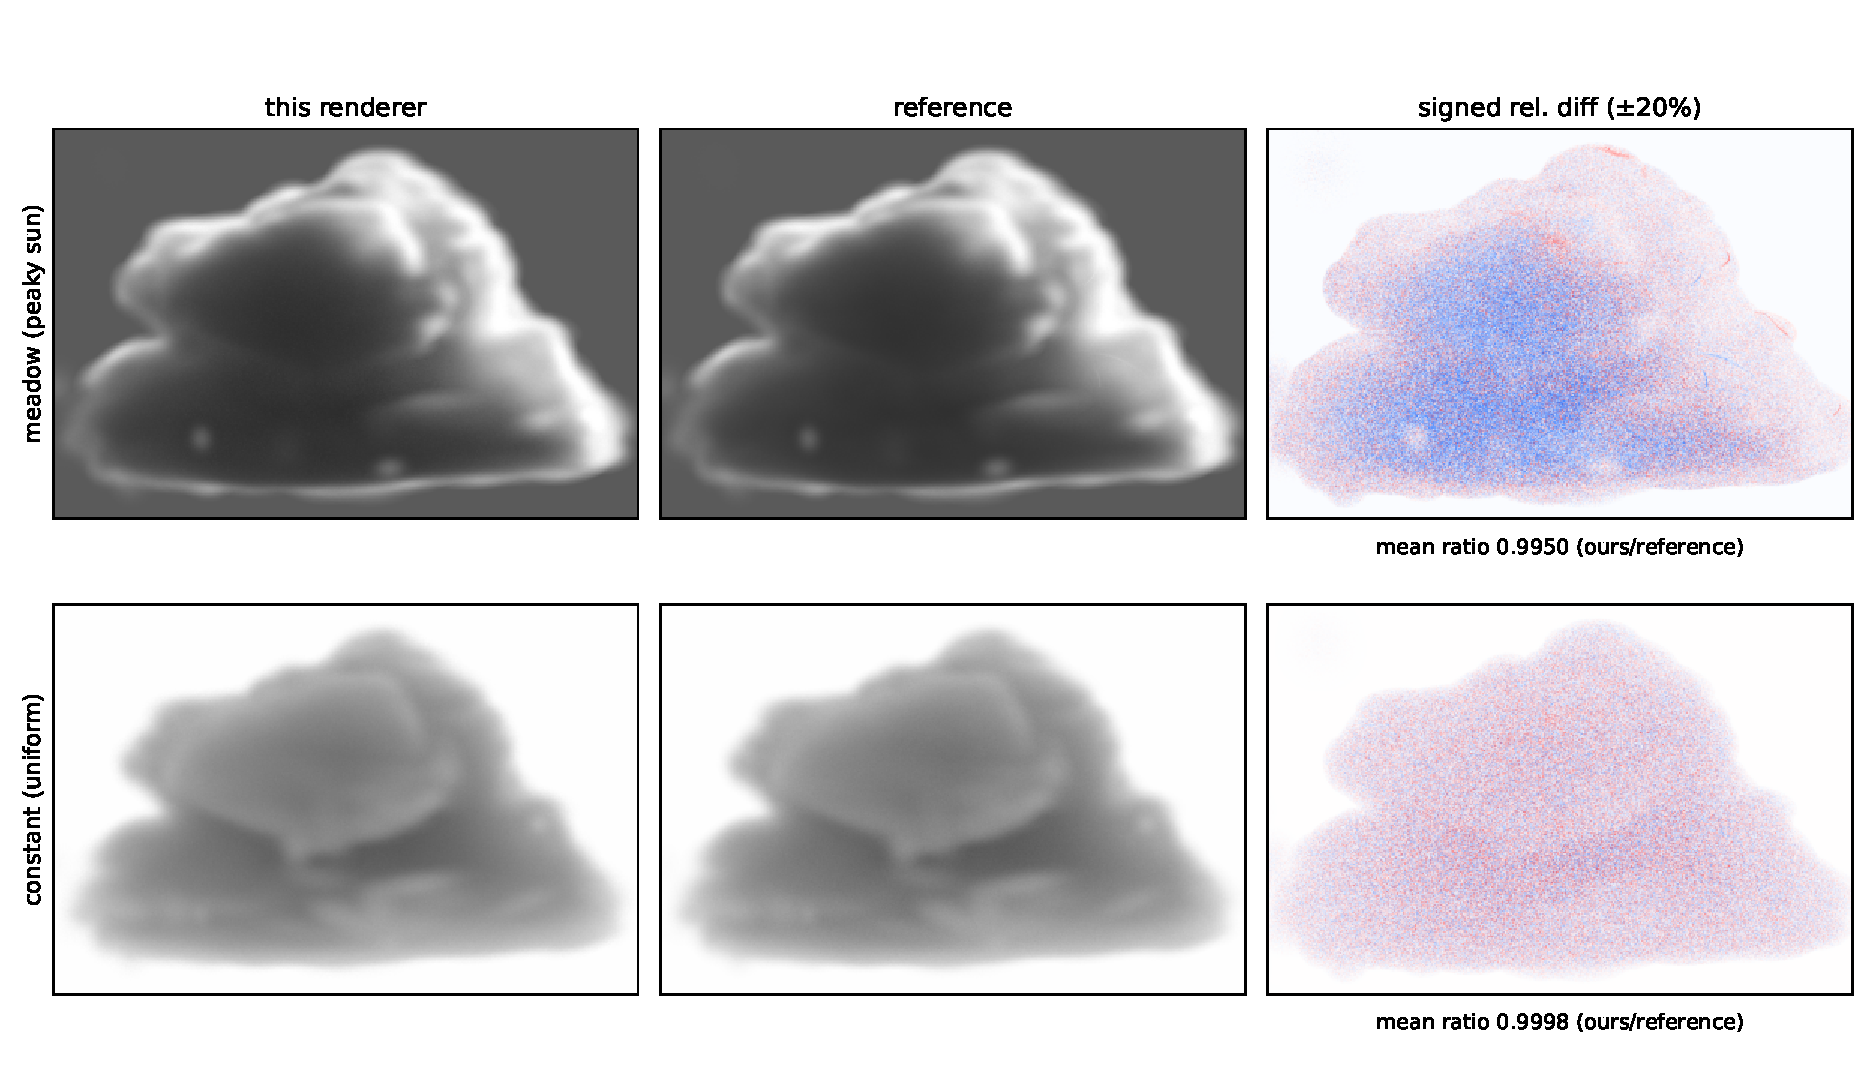
\includegraphics[width=\linewidth]{figures/agreement_panels.pdf}
  \caption{Pixel-level cross-renderer agreement on the cloud, this renderer versus the corrected
  reference (next-event mode), under the peaky meadow environment (\emph{top}) and a uniform
  environment (\emph{bottom}): per-arm renders and the signed relative difference
($\pm\num{20}\,\%$ full scale; conventions, \Cref{sec:setup}). Panels are luminance images: the agreement statistics are computed on luminance
(\Cref{sec:setup}). Budgets: meadow
\num{8}$\times$\num{1024} versus \num{4}$\times$\num{2048}\,spp; uniform
\num{8}$\times$\num{64}\,spp versus a single \num{256}-spp reference render. Tile-level ($60\times60$\,px) readouts: \num{0.67}\,\% coherent excess (meadow) and
${\le}\num{0.07}\,\%$ total (uniform; its single reference render leaves noise and
structure inseparable); the only structure above noise is the deep-shadow region attributed in
\Cref{sec:scattering-ladder} to the reference's shadow-march early-out.}
  \label{fig:agreement-panels}
\end{figure}

\section{Feature validation}
\label{sec:feature-validation}

Each rendering feature is validated against the reference before it is trusted in combination.
The features are environment-map illumination, the Henyey--Greenstein phase function (forward
scattering, $g = 0.85$),
multiple importance sampling, and coloured (non-grey) albedo. \Cref{tab:features}
summarises the gates and their recorded readouts. Each feature matches the reference to
within Monte~Carlo noise, with one exception and one marginal reading. The marginal reading is the cloud-scale environment row: its small global offset
($2.2\sigma$) is within what fireflies produce at that budget. Deciding it would take
several times that budget, and the far-higher-budget pixel-level certification of
\Cref{sec:scattering-ladder} already bounds any real offset in this configuration, so the
gate was not re-run. The exception is
coloured albedo: it leaves a small channel-dependent
residual (smaller than $0.2\,\%$ of the image mean, cause not isolated). It touches only tinted
media; the validation and headline scenes use grey (channel-uniform) albedo. It is the only
\emph{feature-validation} exception, and the second of three small residuals
documented as known limitations (\Cref{ch:conclusion}), alongside the overlap-region
scattering residual of \Cref{sec:scattering-ladder}. The third is a ${+}1.8\times10^{-4}$
brightness offset in low-density interiors. It was measured against Mitsuba-analog at density
scale \num{2} under a constant environment (\num{3} seeds at \num{512}\,spp); it is small but
statistically resolved.

\begin{table}[htp]
  \centering
  \small
  \setlength{\tabcolsep}{3pt}
  \begin{tabular}{@{}>{\raggedright\arraybackslash}p{84pt}
      >{\raggedright\arraybackslash}p{86pt}
      >{\raggedright\arraybackslash}p{58pt}
      >{\raggedright\arraybackslash}p{94pt}@{}}
    \toprule
    Gate & Scene / budget & Readout & Value \\
    \midrule
    Env.\ orientation & single Gaussian, $6$ axis views & RMSE vs reference & $\le 2\times10^{-3}$ (noise floor) \\
    Env.\ lighting, single Gaussian & meadow; $24$v$23 \times 2048$\,spp & mean offset & $(+1.1\pm8.2)\times10^{-4}$ ($0.1\sigma$) \\
    Env.\ lighting, full cloud & meadow; $8$v$8 \times 256$\,spp & mean offset & $(-29\pm13)\times10^{-4}$ ($2.2\sigma$) \\
    \addlinespace[3pt]
    HG phase ($g{=}0.85$), energy & single-Gaussian furnace & furnace bias & $0.5\times10^{-4}$ \\
    HG phase ($g{=}0.85$), agreement & single Gaussian, meadow; $24$ seeds & median $|\Delta|$ & $2.4\times10^{-4}$ \\
    \addlinespace[3pt]
    MIS, energy & single-Gaussian furnace & furnace mean & $1.00011$ \\
    MIS, agreement & meadow; vs phase-IS NEE & mean offset & $+3\times10^{-4}$ ($0.7\sigma$) \\
    \bottomrule
  \end{tabular}
  \caption{Feature-validation gates, one readout per row (development-campaign record). Scenes:
single Gaussian at $\sigma_t$ scale \num{4}, except the cloud row at scale \num{7.5}.
Notation: $a$v$b \times s$ is $a$ seeds of this renderer against $b$ of the reference at
$s$\,spp each (counts need not match; each arm's uncertainty comes from its own spread).
Offsets: absolute radiance $\pm$ standard error. Phase-IS/environment-IS: importance
sampling by the phase function or the environment map. The orientation gate guards a
loader-orientation error class that only full-sphere views can see; coloured albedo is the
documented exception in the text.}
  \label{tab:features}
\end{table}

With the features validated to within the stated residuals, \emph{which} features to enable, and at
what cost in time and quality, becomes a separate question---a performance-engineering one, taken up in
\Cref{ch:optimization}.

\section{The combined showcase}
\label{sec:money-shot}

The features are finally exercised together---the full cloud, under the measured HDR environment, with
forward-scattering Henyey--Greenstein ($g = 0.85$) and MIS direct lighting. Concretely, \emph{the
showcase} throughout this thesis is: the \num{652}-primitive cloud at $\sigma_t$ scale \num{7.5},
albedo \num{0.9}, rendered at $900\times600$ from camera \num{0} of the asset's \num{24}-view ring,
under the \texttt{meadow\_2} environment map (Poly Haven, CC0 public-domain licence, $4096\times2048$). That map is the
``meadow''
of every earlier section; its one dominant light is the sun. Cross-renderer, this
combined configuration agrees with the reference at the Monte-Carlo noise level
(\Cref{fig:agreement-panels}) and to within ${\sim}1\,\%$ across four well-separated views
(\Cref{sec:results-generalisation}). \Cref{fig:showcase} shows the image itself, next to the same
renderer's \emph{analog} mode at the identical sample budget. That pairing is the visual
counterpart of the
direct-lighting variance comparison that \Cref{ch:results} quantifies. This combined result is the
correctness foundation on which the performance study of \Cref{ch:optimization} builds: every optimisation kept there preserves this image; changes that broke it were reverted.

\begin{figure}[htp]
  \centering
  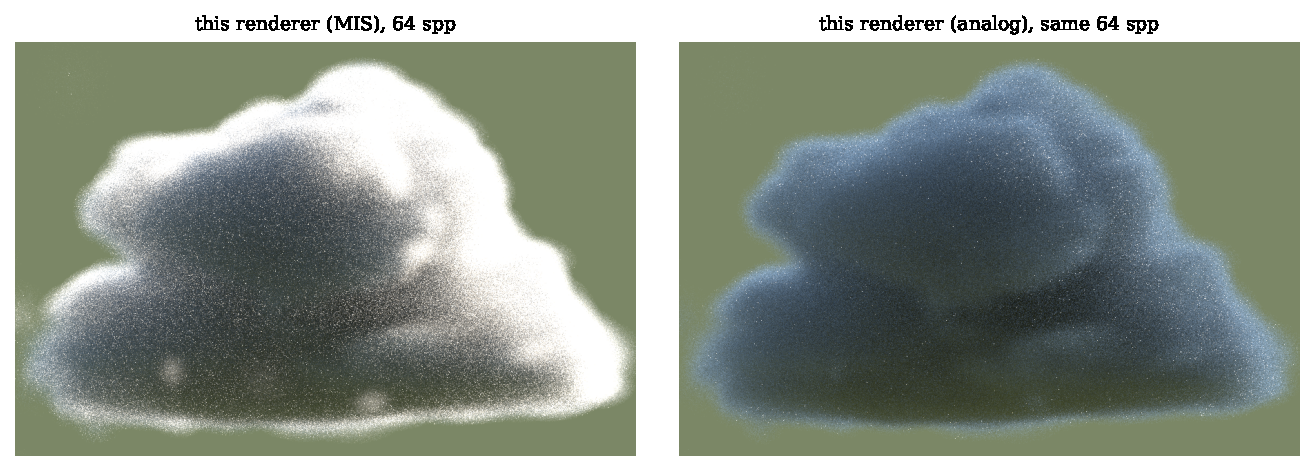
\includegraphics[width=\linewidth]{figures/showcase.pdf}
  \caption{The combined showcase: the full cloud under a measured HDR environment with forward
  Henyey--Greenstein scattering ($g = 0.85$), single \num{64}-spp frames. (The flat khaki backdrop is the environment map itself: the camera is orthographic, so
every ray that misses the cloud samples the map in one single direction, and the backdrop
is that one map value---verified by rendering the environment alone through the same
camera.) \emph{Left:} this renderer's
  production MIS estimator---firefly-free at this budget. \emph{Right:} the same renderer with next-event
  estimation disabled (analog), at the identical budget: the rare bright-sun scattering paths that MIS
  importance-samples become fireflies. The analog frame is also blue-shifted and darker in the body of
  the cloud: the sun's warm energy is concentrated in those rare paths, so at this budget the typical
  pixel sees only the well-sampled blue skylight (per-channel \emph{means} of the two frames agree to
  ${\le}\num{2.1}\,\%$---the colour difference is where the energy sits). The difference is estimator
  \emph{variance}, not bias: both modes are unbiased estimators of the same image, and each
passes the furnace test of \Cref{fig:furnace-four}. The equal-quality cost is quantified
in \Cref{ch:results}.}
  \label{fig:showcase}
\end{figure}
